
\paragraph{Recap.} We keep the notation of the last lecture ($a$, $b = N - a$ with
$1 \leq a \leq N - 1$, $\ket{A}$, $\ket{B}$, $Z_f$, $Z_0$, $D$, $\ket{h}$ and the Grover iteration
$G = D Z_f = -H^{\otimes n} Z_0 H^{\otimes n} Z_f$; \cref{fig:grover-circuit-1006}). By
\cref{eq:h-AB-1006}, $\ket{h} = \sin\theta \ket{A} + \cos\theta \ket{B}$ with
$\theta = \sin^{-1}\left(\sqrt{\sfrac{a}{N}}\right) \in (0, \sfrac{\pi}{2})$. We write a unit vector
of the plane spanned by $\ket{A}$ and $\ket{B}$ with real coefficients as
$\sin\alpha \ket{A} + \cos\alpha \ket{B}$ and call $\alpha$ its \emph{angle} (measured from $\ket{B}$
towards $\ket{A}$). So $\ket{h}$ has angle $\theta$, and a measurement of the state with angle
$\alpha$ gives a solution with probability $\sin^2\alpha$.

\section{A Grover Iteration Is Two Reflections}

Since $Z_f \ket{A} = -\ket{A}$ and $Z_f \ket{B} = \ket{B}$ (proof of \cref{lem:giter-1006}),
$Z_f \left(\sin\alpha \ket{A} + \cos\alpha \ket{B}\right) = \sin(-\alpha) \ket{A} + \cos(-\alpha) \ket{B}$.
So $Z_f$ is the reflection of the plane about the line of $\ket{B}$.

Let $\ket{h^\perp} = \cos\theta \ket{A} - \sin\theta \ket{B}$. It is a unit vector of the plane with
$\braket{h}{h^\perp} = \sin\theta\cos\theta - \cos\theta\sin\theta = 0$, so $\ket{h}$ and
$\ket{h^\perp}$ are a second orthonormal basis of the plane (\cref{fig:reflections-1008}).

\begin{exercisebox}
\begin{exercise}\label{ex:diffusion-1008}
    Show that $D = 2\ket{h}\bra{h} - I$, and that for every state
    $\ket{\phi} = c \ket{h} + d \ket{h^\perp}$ of the plane,
    \[D \ket{\phi} = c \ket{h} - d \ket{h^\perp}.\]
\end{exercise}
\tcblower
\begin{wsolution}
    The first claim is \cref{lem:diffusion-1006}: $H^{\otimes n} H^{\otimes n} = I$ and
    $\bra{0^n} H^{\otimes n} = \bra{h}$ give
    \[D = -H^{\otimes n}\left(I - 2\ket{0^n}\bra{0^n}\right)H^{\otimes n} = 2\ket{h}\bra{h} - I.\]
    Since $\braket{h}{h} = 1$ and $\braket{h}{h^\perp} = 0$, we have $\braket{h}{\phi} = c$, so
    \[D\ket{\phi} = 2\ket{h}\braket{h}{\phi} - \ket{\phi} = 2c\ket{h} - c\ket{h} - d\ket{h^\perp}
        = c\ket{h} - d\ket{h^\perp}.\]
    So $D$ is the reflection of the plane about the line of $\ket{h}$.
\end{wsolution}
\end{exercisebox}

\begin{figure}[ht]
    \centering
    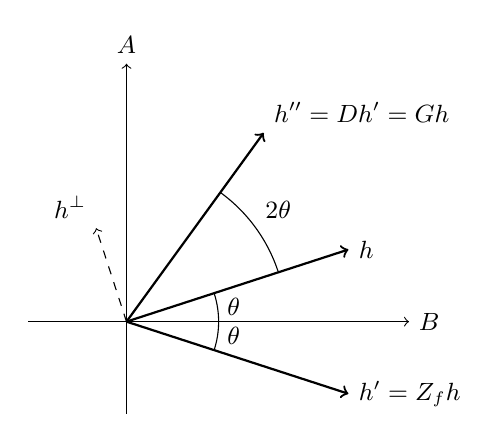
\begin{tikzpicture}[scale=0.78, every node/.style={font=\small}]
        \draw[->] (-1.6,0) -- (4.6,0) node[right] {$\ket{B}$};
        \draw[->] (0,-1.5) -- (0,4.2) node[above] {$\ket{A}$};
        \draw[->, thick] (0,0) -- (18:3.8) node[right] {$\ket{h}$};
        \draw[->, thick] (0,0) -- (-18:3.8) node[right] {$\ket{h'} = Z_f\ket{h}$};
        \draw[->, thick] (0,0) -- (54:3.8) node[above right] {$\ket{h''} = D\ket{h'} = G\ket{h}$};
        \draw[->, dashed] (0,0) -- (108:1.6) node[above left] {$\ket{h^\perp}$};
        \draw (1.5,0) arc (0:18:1.5) node[midway, right] {$\theta$};
        \draw (1.5,0) arc (0:-18:1.5) node[midway, right] {$\theta$};
        \draw (18:2.6) arc (18:54:2.6) node[midway, above right] {$2\theta$};
    \end{tikzpicture}
    \caption{One Grover iteration applied to $\ket{h}$: $Z_f$ reflects about the line of $\ket{B}$,
        then $D$ reflects about the line of $\ket{h}$.}
    \label{fig:reflections-1008}
\end{figure}

\subsection{Two Reflections Make a Rotation}

In \cref{fig:reflections-1008} the first reflection takes the angle $\theta$ to $-\theta$ and the
second, about the line at angle $\theta$, takes $-\theta$ to $3\theta$.

\begin{claim}[Two Reflections Make a Rotation]\label{lem:tworef-1008}
    Let $\ket{A}$ and $\ket{B}$ be orthonormal vectors, let $\theta$ be a real number and
    $\ket{\psi} = \sin\theta \ket{A} + \cos\theta \ket{B}$. Let $S$ be a linear operator with
    $S\ket{A} = -\ket{A}$ and $S\ket{B} = \ket{B}$, and let $T = 2\ket{\psi}\bra{\psi} - I$. Then for
    every real number $\beta$,
    \[T S \left(\sin\beta \ket{A} + \cos\beta \ket{B}\right)
        = \sin(\beta + 2\theta) \ket{A} + \cos(\beta + 2\theta) \ket{B},\]
    and so, for every integer $k \geq 0$,
    \[(TS)^k \ket{\psi} = \sin\left((2k+1)\theta\right) \ket{A} + \cos\left((2k+1)\theta\right) \ket{B}.\]
\end{claim}

\begin{proof}
    By linearity, $S(\sin\beta \ket{A} + \cos\beta \ket{B}) = -\sin\beta \ket{A} + \cos\beta \ket{B}
        = \sin\gamma \ket{A} + \cos\gamma \ket{B} =: \ket{\chi}$ with $\gamma = -\beta$. By orthonormality,
    $\braket{\psi}{\chi} = \sin\theta\sin\gamma + \cos\theta\cos\gamma = \cos(\gamma - \theta)$, so
    \begin{align*}
        T\ket{\chi} & = 2\cos(\gamma - \theta)\ket{\psi} - \ket{\chi}                                     \\
                    & = \left(2\cos(\gamma - \theta)\sin\theta - \sin\gamma\right)\ket{A}
        + \left(2\cos(\gamma - \theta)\cos\theta - \cos\gamma\right)\ket{B}.
    \end{align*}
    By the product formulas $2\cos u \sin v = \sin(u + v) - \sin(u - v)$ and
    $2\cos u \cos v = \cos(u + v) + \cos(u - v)$ with $u = \gamma - \theta$ and $v = \theta$, the
    coefficients are $-\sin(\gamma - 2\theta) = \sin(2\theta - \gamma)$ and
    $\cos(\gamma - 2\theta) = \cos(2\theta - \gamma)$. So $T$ sends the angle $\gamma$ to
    $2\theta - \gamma$, and $TS$ sends $\beta$ to $2\theta - (-\beta) = \beta + 2\theta$. This is the
    first claim. The state $\ket{\psi}$ has the angle $\theta$ and each application of $TS$ adds
    $2\theta$, so induction on $k$ gives the angle $(2k+1)\theta$ for $(TS)^k\ket{\psi}$.
\end{proof}

For Grover's algorithm we take $S = Z_f$, $\ket{\psi} = \ket{h}$ and $T = D = 2\ket{h}\bra{h} - I$
(\cref{ex:diffusion-1008}), so that $TS = D Z_f = G$:

\begin{corollary}[The State After $k$ Iterations]\label{cor:hk-1008}
    Every Grover iteration rotates the plane by $2\theta$ from $\ket{B}$ towards $\ket{A}$, and the
    state after $k$ iterations is
    \[\ket{h^k} = G^k\ket{h} = \sin\left((2k+1)\theta\right) \ket{A} + \cos\left((2k+1)\theta\right) \ket{B}.\]
    A measurement of $\ket{h^k}$ gives a solution with probability $\sin^2\left((2k+1)\theta\right)$.
\end{corollary}

\subsection{The Matrix of a Grover Iteration}

Let $M$ be the matrix of the Grover iteration in the basis $(\ket{B}, \ket{A})$
(\cref{eq:gmatrix-1006}).

\begin{exercisebox}
\begin{exercise}\label{ex:msquare-1008}
    Show that
    \[M = \begin{pmatrix} \sqrt{\sfrac{b}{N}} & -\sqrt{\sfrac{a}{N}} \\[1ex] \sqrt{\sfrac{a}{N}} & \sqrt{\sfrac{b}{N}} \end{pmatrix}^{2}
        = \begin{pmatrix} \cos\theta & -\sin\theta \\ \sin\theta & \cos\theta \end{pmatrix}^{2},\]
    that is, the Grover iteration is the rotation by $\theta$ applied twice.
\end{exercise}
\tcblower
\begin{wsolution}
    Let $R_\theta = \left(\begin{smallmatrix} \cos\theta & -\sin\theta \\ \sin\theta & \cos\theta \end{smallmatrix}\right)$
    with $\cos\theta = \sqrt{\sfrac{b}{N}}$ and $\sin\theta = \sqrt{\sfrac{a}{N}}$. Multiplying,
    \[R_\theta^2
        = \begin{pmatrix} \cos^2\theta - \sin^2\theta & -2\sin\theta\cos\theta \\ 2\sin\theta\cos\theta & \cos^2\theta - \sin^2\theta \end{pmatrix}
        = \begin{pmatrix} \dfrac{b - a}{N} & -\dfrac{2\sqrt{ab}}{N} \\[2ex] \dfrac{2\sqrt{ab}}{N} & \dfrac{b - a}{N} \end{pmatrix} = M,\]
    and by the double angle formulas the middle matrix is $R_{2\theta}$. So $M^k = R_{2k\theta}$.
    This is \cref{cor:hk-1008} in matrix form: $\ket{h}$ is the first column
    $(\cos\theta, \sin\theta)^T$ of $R_\theta$, so $M^k\ket{h}$ is the first column of $R_{(2k+1)\theta}$.
\end{wsolution}
\end{exercisebox}

\section{The Number of Iterations}\label{sec:iterations-1008}

By \cref{cor:hk-1008} we want $(2k+1)\theta \approx \sfrac{\pi}{2}$, so we take $k$ to be an integer
closest to $\frac{\pi}{4\theta} - \frac{1}{2}$. Since $\theta \approx \sin\theta = \sqrt{\sfrac{a}{N}}$
for small $\sfrac{a}{N}$, this is
\[k \approx \frac{\pi}{4}\sqrt{\frac{N}{a}}, \qquad \text{for a unique solution} \quad k \approx \frac{\pi}{4}\sqrt{N}.\]

\begin{exercisebox}
\begin{exercise}\label{ex:iterations-1008}\label{thm:iterations-1008}
    Let $f$ have $a$ solutions, $1 \leq a \leq N - 1$, and let $k$ be an integer closest to
    $\frac{\pi}{4\theta} - \frac{1}{2}$. Show that Grover's algorithm with $k$ iterations outputs a
    solution with probability at least $1 - \sfrac{a}{N}$.
\end{exercise}
\tcblower
\begin{proof}
    Let $t = \frac{\pi}{4\theta} - \frac{1}{2}$, so that $(2t+1)\theta = \sfrac{\pi}{2}$. Then
    $\abs{k - t} \leq \sfrac{1}{2}$ and
    \[(2k+1)\theta = \frac{\pi}{2} + 2(k-t)\theta, \qquad \abs{2(k-t)\theta} \leq \theta.\]
    By \cref{cor:hk-1008} and $\sin(\sfrac{\pi}{2} + x) = \cos x$, the success probability is
    \[\sin^2\left((2k+1)\theta\right) = \cos^2\left(2(k-t)\theta\right) \geq \cos^2\theta = 1 - \frac{a}{N},\]
    because the cosine is even and decreases on $[0, \sfrac{\pi}{2}]$, and $\sin^2\theta = \sfrac{a}{N}$.
\end{proof}
\end{exercisebox}

\section{A Random Number of Iterations}\label{sec:randomk-1008}

The number of iterations, about $\frac{\pi}{4}\sqrt{\sfrac{N}{a}}$, depends on the number $a$ of
solutions, which we may not know. So we choose $k$ \emph{at random}. Since $\sqrt{N}$ need not be an
integer, the largest value is $\floor{2\sqrt{N}}$.

\begin{exercisebox}
\begin{exercise}\label{ex:randomk-1008}\label{thm:randomk-1008}
    Let $N = 2^n$, let $f$ have $a$ solutions, $1 \leq a \leq \sfrac{N}{2}$, and let
    $K = \floor{2\sqrt{N}}$. Choose $k$ uniformly at random from $\set{1, \dots, K}$, make $k$ Grover
    iterations on $\ket{h}$ and measure. Prove that the probability of measuring a solution is
    \begin{equation}\label{eq:avg-1008}
        \prob{\text{success}} = \frac{1}{2} - \frac{\sin\left(4(K+1)\theta\right) - \sin 4\theta}{4K\sin 2\theta}
        \geq \frac{1}{2} - \frac{1}{4K\sin 2\theta} \geq \frac{3}{8},
    \end{equation}
    so that $\prob{\text{success}} = \bigTh{1}$ with at most $2\sqrt{N} = \bigO{\sqrt{N}}$ queries.
\end{exercise}
\tcblower
\begin{proof}
    \emph{The average.} Given $k$, the success probability is $\sin^2((2k+1)\theta)$ by
    \cref{cor:hk-1008}, and each value has probability $\sfrac{1}{K}$. By the law of total probability
    and $\sin^2 x = \frac{1}{2}(1 - \cos 2x)$,
    \[\prob{\text{success}} = \frac{1}{K}\sum_{k=1}^{K} \sin^2\left((2k+1)\theta\right)
        = \frac{1}{2} - \frac{1}{2K}\sum_{k=1}^{K} \cos\left((4k+2)\theta\right).\]
    By the product formula $2\cos u \sin v = \sin(u+v) - \sin(u-v)$ with $u = (4k+2)\theta$ and
    $v = 2\theta$, the sum telescopes:
    \[2\sin 2\theta \sum_{k=1}^{K} \cos\left((4k+2)\theta\right)
        = \sum_{k=1}^{K} \left(\sin\left(4(k+1)\theta\right) - \sin\left(4k\theta\right)\right)
        = \sin\left(4(K+1)\theta\right) - \sin 4\theta.\]
    As $\sin\theta = \sqrt{\sfrac{a}{N}} \leq \sfrac{1}{\sqrt{2}}$, we have $0 < \theta \leq \sfrac{\pi}{4}$
    and $\sin 2\theta > 0$, so dividing by $2\sin 2\theta$ gives the equality in \cref{eq:avg-1008}.

    \emph{The lower bound.} $\sin(4(K+1)\theta) \leq 1$, and $\sin 4\theta \geq 0$ because
    $0 < 4\theta \leq \pi$. So the numerator is at most $1$, which gives the first inequality in
    \cref{eq:avg-1008}. Since $b = N - a \geq \sfrac{N}{2}$,
    \[\sin 2\theta = 2\sin\theta\cos\theta = \frac{2\sqrt{ab}}{N} \geq \frac{2\sqrt{a \cdot \sfrac{N}{2}}}{N} = \sqrt{\frac{2a}{N}}.\]
    Next, $\floor{2\sqrt{N}} \geq \sqrt{2N}$ for $N = 2^n$. If $n$ is even, $2\sqrt{N}$ is an integer.
    If $n$ is odd, $\sqrt{2N} = 2^{(n+1)/2}$ is an integer with $\sqrt{2N} \leq 2\sqrt{N}$, so it is at
    most the floor. So $K\sin 2\theta \geq \sqrt{2N} \cdot \sqrt{\sfrac{2a}{N}} = 2\sqrt{a} \geq 2$
    and $\prob{\text{success}} \geq \frac{1}{2} - \frac{1}{8} = \frac{3}{8}$. A probability is at most
    $1$, so $\prob{\text{success}} = \bigTh{1}$. The number of queries is $k \leq K \leq 2\sqrt{N}$.
\end{proof}
\end{exercisebox}

For the set $\set{1, \dots, \floor{\sqrt{N}}}$ the same proof with
$K = \floor{\sqrt{N}} \geq \sqrt{\sfrac{N}{2}}$ gives $\prob{\text{success}} \geq \sfrac{1}{4}$.

\section{Quantum Amplitude Amplification}\label{sec:ampamp-1008}

Let $\mathcal{A}$ be any quantum algorithm without measurements (a unitary operator on $n$
qubits), and let $f \colon \set{0,1}^n \to \set{0,1}$ tell us which outcomes $x$ are \emph{good}
($f(x) = 1$) and which are \emph{bad} ($f(x) = 0$). Write
$\mathcal{A}\ket{0^n} = \sum_x c_x \ket{x}$, let
$p = \sum_{x \suchthat f(x) = 1} \abs{c_x}^2$ be the probability that a measurement of
$\mathcal{A}\ket{0^n}$ gives a good outcome, and assume $0 < p < 1$. With the unit vectors
\[\ket{G} = \frac{1}{\sqrt{p}} \sum_{x \suchthat f(x) = 1} c_x \ket{x},
    \qquad
    \ket{B} = \frac{1}{\sqrt{1-p}} \sum_{x \suchthat f(x) = 0} c_x \ket{x},\]
which are orthogonal because no basis state appears in both, the state that $\mathcal{A}$ produces is
$\ket{\phi} = \mathcal{A}\ket{0^n} = \sqrt{p}\, \ket{G} + \sqrt{1-p}\, \ket{B}$. Here $\ket{G}$ is
the good state, unrelated to the Grover iteration $G$.
\emph{Classically} we would run $\mathcal{A}$, measure, check the outcome with $f$, and repeat until
the outcome is good. The number of runs is geometric with mean $\sfrac{1}{p}$.

\begin{exercisebox}
\begin{exercise}\label{ex:ampamp-1008}\label{thm:ampamp-1008}
    Let $\theta \in (0, \sfrac{\pi}{2})$ with $\sin\theta = \sqrt{p}$, and let
    \[Q = -\mathcal{A} Z_0 \mathcal{A}^{-1} Z_f.\]
    Show that
    $Q^k\ket{\phi} = \sin\left((2k+1)\theta\right)\ket{G} + \cos\left((2k+1)\theta\right)\ket{B}$
    for every $k \geq 0$. Show that for $k = \floor{\sfrac{\pi}{4\theta}}$, a measurement of
    $Q^k\ket{\phi}$ gives a good outcome with probability at least $\max(p, 1 - p) \geq \sfrac{1}{2}$,
    and that computing $Q^k \mathcal{A}\ket{0^n}$ takes
    $2k + 1 \leq \frac{\pi}{2\sqrt{p}} + 1 = \bigO{\sfrac{1}{\sqrt{p}}}$ applications of $\mathcal{A}$ or
    $\mathcal{A}^{-1}$ and $k$ queries to $f$.
\end{exercise}
\tcblower
\begin{proof}
    $Z_f\ket{G} = -\ket{G}$ and $Z_f\ket{B} = \ket{B}$. Since $\mathcal{A}$ is unitary,
    $\bra{0^n}\mathcal{A}^{-1} = \left(\mathcal{A}\ket{0^n}\right)^\dagger = \bra{\phi}$, so
    \[-\mathcal{A} Z_0 \mathcal{A}^{-1} = -\mathcal{A}\left(I - 2\ket{0^n}\bra{0^n}\right)\mathcal{A}^{-1}
        = 2\ket{\phi}\bra{\phi} - I.\]
    So $Q$ is the reflection about $\ket{B}$ followed by the reflection about
    $\ket{\phi} = \sin\theta\ket{G} + \cos\theta\ket{B}$, and \cref{lem:tworef-1008} gives the formula
    for $Q^k\ket{\phi}$.

    $\ket{G}$ contains only good basis states and $\ket{B}$ only bad ones, so the success
    probability is $\sin^2((2k+1)\theta)$. For $k = \floor{\sfrac{\pi}{4\theta}}$ we have
    $\frac{\pi}{2} - \theta < (2k+1)\theta \leq \frac{\pi}{2} + \theta$, so it is at least
    $\cos^2\theta = 1 - p$. If $p \leq \sfrac{1}{2}$, then $1 - p = \max(p, 1-p)$. If
    $p > \sfrac{1}{2}$, then $\theta > \sfrac{\pi}{4}$, so $k = 0$ and it is $\sin^2\theta = p$.

    Each application of $Q$ uses $\mathcal{A}$ once, $\mathcal{A}^{-1}$ once and one query to $f$, and
    preparing $\ket{\phi}$ uses $\mathcal{A}$ once more. So the cost is $2k + 1$ applications and
    $k$ queries. Since $\sin\theta \leq \theta$, $k \leq \frac{\pi}{4\theta} \leq \frac{\pi}{4\sqrt{p}}$,
    so $2k + 1 \leq \frac{\pi}{2\sqrt{p}} + 1$.
\end{proof}
\end{exercisebox}
